\documentclass[a4paper,12pt]{report}

\usepackage{alltt, fancyvrb, url}
\usepackage{graphicx}
\usepackage[utf8]{inputenc}
\usepackage{float}
\usepackage{hyperref}

% Questo commentalo se vuoi scrivere in inglese.
\usepackage[italian]{babel}

\usepackage[italian]{cleveref}

\title{Relazione Assignment-01 \\ per l'esame \\ ``Programmazione Concorrente e distribuita''}
\author{Rattini Emiliano\\Giosuè Giocondo Mainardi}

\date{\today}


\begin{document}

\maketitle

\tableofcontents

\chapter{Analisi}
% A brief analsysis of the problem, focusing in particular aspects that are relevant from concurrent point of view.

\chapter{Design}
% A description of the adopted design, the strategy and architecture.

\chapter{Comportamento}
% A description of the behaviour of the system using one or multiple Petri Nets, choosing the propor level of abstraction.

\chapter{Test di performance}
% Performance tests, to analyse and discuss the performance of the programs (for each version) compared to the sequential version

\chapter{Verifica con JPF}
% Verification of the program (a model of it) using JPF. For this point, only the Java multithreaded programming version may be considered.

\chapter{Esempi di utilizzo}
Esempio di immagine inserita sul posto.
\begin{figure}[h]
\centering{}
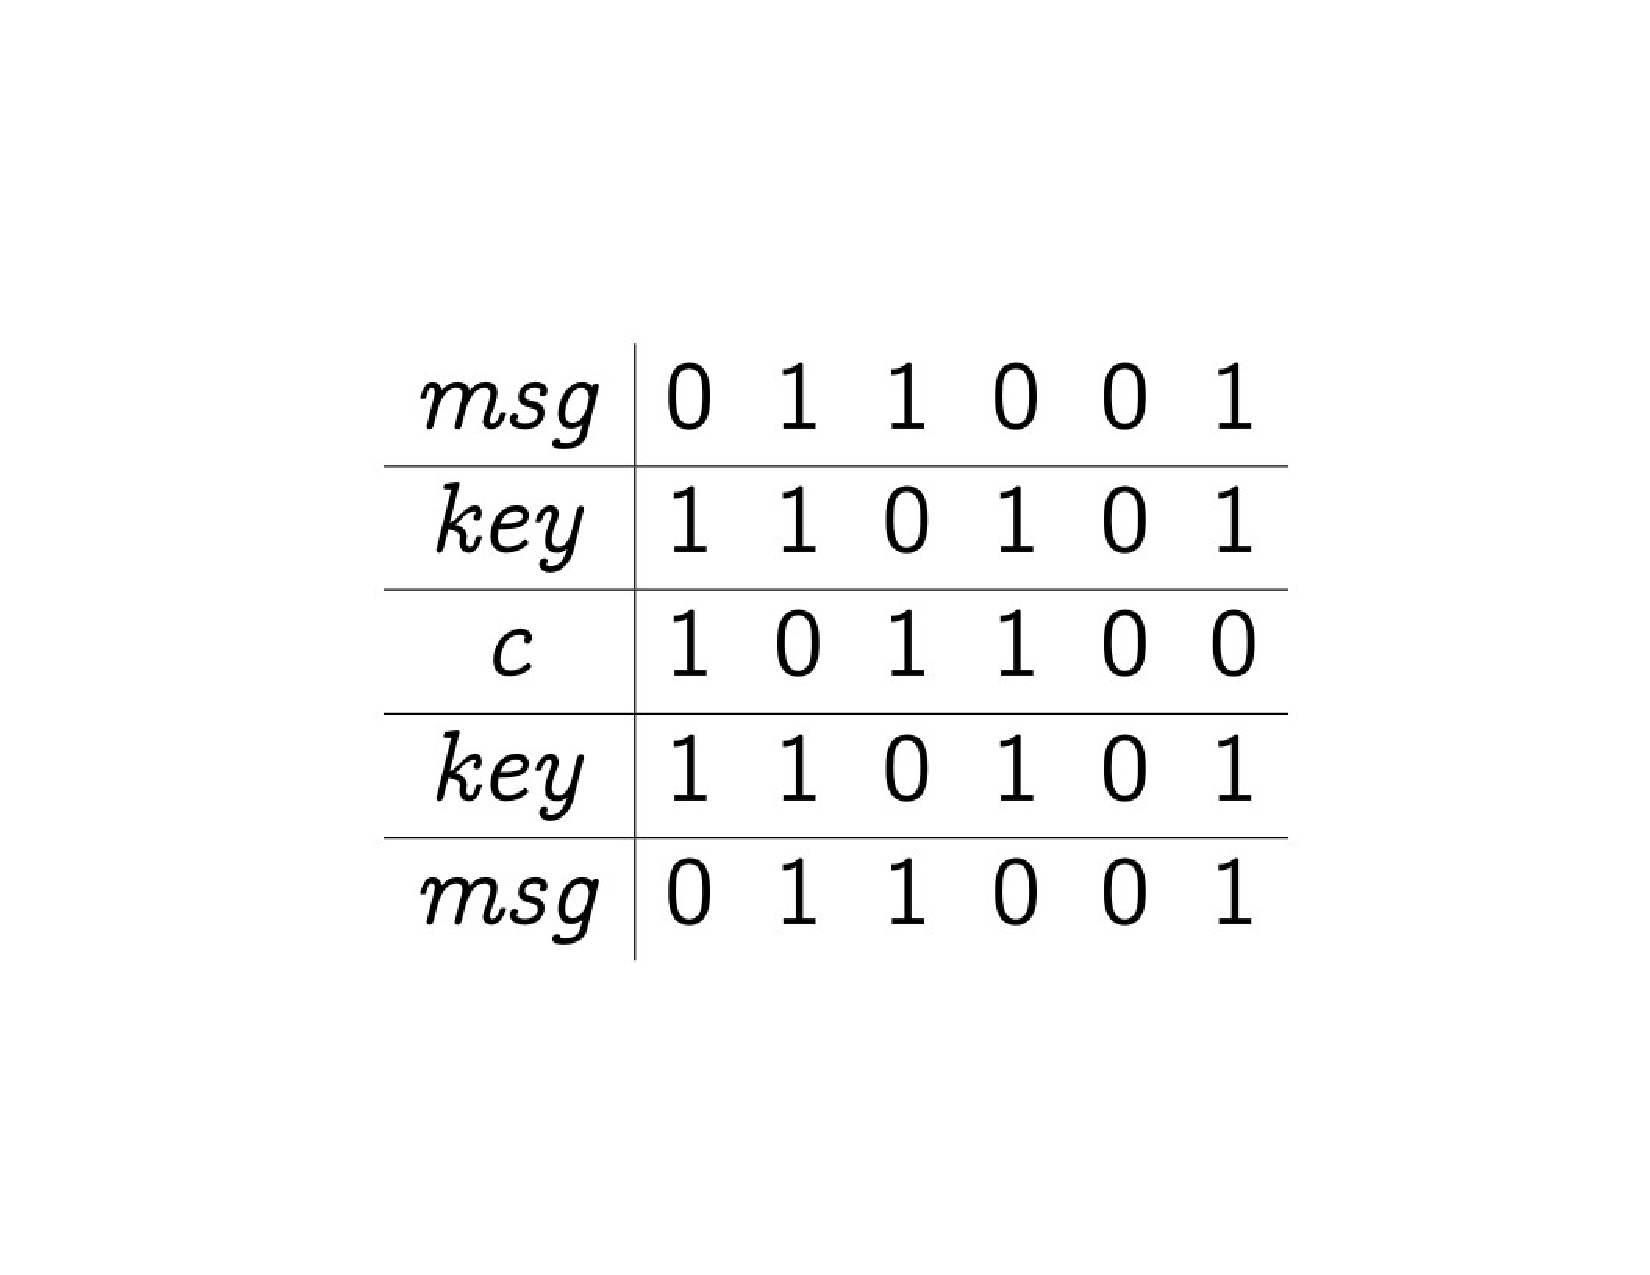
\includegraphics[width=\textwidth]{img/example_img.pdf}
\caption{L'interfaccia \texttt{GLaDOS}.}
\label{img:example}
\end{figure}

\paragraph{Paragrafo Risposta 1} Contenuto \textit{paragrafo}, con riferimento immagine
\Cref{img:example}: e anche \texttt{Scrittura unicode}.

Esempio di link
Permalink: \url{https://github.com/AlchemistSimulator/Alchemist/blob/d8a1799027d7d685569e15316a32e6394632ce71/alchemist-incarnation-protelis/src/main/java/it/unibo/alchemist/protelis/AlchemistExecutionContext.java#L141-L143}

% \appendix
% \chapter{Capitolo appendice 1}

% Contenuto.

% \chapter{Capitolo appendice 2}

% Contenuto.

\bibliographystyle{alpha}
\bibliography{report-template}

\end{document}
